\chapter{Introduction}

\atrcomments{TBD!!}

Syntactic parsing refers to the process of extracting and analyzing the syntactic structure or representation of a natural language text. This is very useful is a variety of different domains such as machine translation, information retrieval, question answering \cite{hall2008transition}. More formally, we can define it as a structural prediction problem. Hence, there is an input which are sentences; an output, which are syntactic representation of a sentence;  and a model that maps the input to the output. The input sentence is usually split into tokens. The output is represented as trees. Dependency parsing is a type of syntactic parsing analyses the dependency structure of a sentence based on a dependency grammar. As illustrated in figure~\ref{fig:depParsetree}, the words in a sentence are linked with relations (shown using labeled arrows), also known as dependency relation (dependencies) where one word is the dependent~\footnote{can also be referred to as child} which depends on the head~\footnote{can also be referred to as parent}. In order to simplify the problem to provide a syntactic head to the word which does not have a head, an artificial root is introduced~\cite{kubler2009dependency}. Dependency parsing gained prominence because of the flexibility it provides for free word order languages such as Czech.

Most commonly used dependency parsing approaches are transition-based and graph-based. The transition based approach is a greedy locally optimized classifier that learns how to get from one parse state to the next. %For dependency parsing, each step represents the steps for deriving the final dependency tree. These are stack-based and there are usually three different kinds of transitions - shift, left \& right which are chosen based on an oracle, usually a machine learning classifier such as SVM. 
In contrast, for graph-based dependency parsing, the problem lies in finding maximum spanning trees (MST). The MST parser is state of the art in graph based parsing. The core idea of the parser to compute a score of the dependency tree~\footnote{Score of the tree is the sum of the score of each edge of the tree} which is a dot product of weight and a high dimensional feature vector. %Thus, it can be thought of as a problem of multiclass classification, where each dependency tree of the sentence is a class. 
The resulting dependency parse is the highest scoring tree. I use MATE~\cite{bohnet2010very}~\footnote{code.google.com/p/mate-tools} which is a reimplementation of MST parser~\cite{McDonald:2005:NDP:1220575.1220641} for my experiments. %MATE parallelizes the feature extraction and parsing algorithm by using passive-aggressive perceptron algorithm~\cite{crammer2006online} as Hash Kernel. 
The parser is highly efficient in terms of memory utilization and CPU requirements while maintaining the accuracy of the resultant parses.
%Bohnet reported a 3.5 times increase in speed over the baseline MST parser using a single core CPU and it also requires a lot less memory than the contemporary parsers by using Hash Kernel. The speed increases further by using parallel algorithms and it can be further reduced at the cost of accuracy.

\begin{figure*}[!htb]
    \centering
    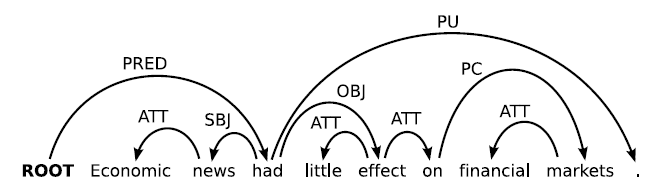
\includegraphics[scale = 0.6]{figures/dep-tree.png}
    \centering
    \caption{Dependency parsing tree~\cite{kubler2009dependency}}
    \label{fig:depParsetree}
\end{figure*}

Part of speech (POS) tagging refers to finding part of speech tags (e.g., nouns, verbs, adjectives) in a sentence. Often POS tagging is a precursor step in parsing, which is why, I look at POS tagging in my experiments, as well. These tasks generally work well when applied on the dataset from the same domain. However, the performance suffers when source and target are from different domains. The work in the area is largely driven by unavailability of data from the target domain. It is nearly impossible to hand annotate the huge amount of data generated by various sources. Manual annotation is even harder when the syntactic structure of the data differs widely. E.g., the syntactic structure of a newspaper corpus is very different from that of social media or academic journals from biomedical domain or literary works. This is an interesting problem since a deep understanding of syntactic structure of a sentence helps in variety of NLP tasks such as question answering, sentiment analysis, opinion mining, etc. Dependency parsing is particularly useful because the dependency relations serve as an important feature to detect negation or multi word expressions, for instance. 
